\documentclass[12pt,a4paper,twoside]{article}
\usepackage[english]{babel}
\usepackage{parskip}
\usepackage{bibentry}
\usepackage{afterpage}

\begin{document}

\begin{center}
	\Large
	Computer Science Tripos -- Part II -- Project Proposal\\[4mm]
	\LARGE
	Framework for empirical analysis of graph metric robustness\\[4mm]
	
	\large
	Juraj~Mi\v{c}ko, Jesus College

	Originator: Dr Timothy Griffin

	25 October 2019
\end{center}

\vspace{5mm}

\textbf{Project Supervisor:} Dr Timothy Griffin

\textbf{Director of Studies:} Dr Christopher Town

\textbf{Project Overseers:} Dr Rafal Mantiuk, Prof Andrew Pitts

\section*{Introduction}

	There exist numerous graphs representing the real world, such as proteins and their interactions, social networks, citation networks, web graphs, road networks and more. Those graphs are huge so are often analysed and described by studying different metrics (i.e. functions of graphs or graph nodes such as radius, degree, betweenness centrality, etc.; not necessarily numerical). Some graph databases provide edge weights indicating the available experimental evidence or confidence. Further networks are then built by thresholding on these weights, which is sensitive to the choice of such threshold.

    In my work, I will study and compare ways to obtain multiple graphs of the similar nature; define and analyse 'robustness' of graph metrics when applied to such graphs, i.e. study how sensitive to some perturbations in the input graph these metrics are; and evaluate which graph metrics are better suited for describing graphs of respective application areas. As an extension to a standalone project, this can be turned into a library or a plugin to the graph visualisation software Gephi.

\section*{Starting point}

    The idea of this project stems from the following research paper:
    
    \begin{adjustwidth}{1cm}{}
    Bozhilova, L. V., Whitmore, A. V., Wray, J., Reinert, G., \& Deane, C. M. (2019). Measuring rank robustness in scored protein interaction networks. BMC Bioinformatics, 20(1). \url{https://doi.org/10.1186/s12859-019-3036-6}
    \end{adjustwidth}
    
    The study discusses at a few possible ways to analyse robustness of graph metrics specifically on protein graphs consisting of weighted edges. The authors came up with three different measures of robustness of a \textit{graph metric applied to a graph within a specific confidence range}: Rank continuity, Rank identifiability, Rank instability, three different ways to assess how much the metric values change when changing the threshold. The weight of an edge between two proteins signals the amount of evidence for the specific protein interaction. Methods in this research paper require graphs with such weights, but the idea of metric robustness could be generalised.

    There exist numerous libraries for working with graphs, such as Apache Giraph, JGraphT, JUNG and others, each having a different focus: iterative graph processing, algorithms, visualisation and others. I plan to base the project on one of such libraries and extend it by implementing various algorithms for computing graph metrics. I will also decide on a~way to store the graphs in the file system.
    
    I have theoretical knowledge of Java, algorithms, data science and other relevant topics from respective courses from the Computer Science Tripos. I also have some practical and software engineering skills from the Part IB project, my internships and other personal projects. I will need to study a lot of materials about graphs, networks, graph metrics, algorithms and similar topics.
    
    This project will also use graph datasets from sources mentioned in~\nameref{sec:resourcedeclaration}.

\section*{Work to be done}

    \subsection*{Robustness}

    	The goal of this project is to devise, study and compare 'robustness' of graph metrics when applied to specific graphs and conclude whether some metrics are more robust than others for describing particular types of graphs. The essence of this project is primarily the experiment itself and the concluding comparison of graph metrics rather than the platform needed to perform such an experiment.
    	
    \subsection*{Generate graphs}
    	
    	In order to test the robustness, a metric has to be evaluated over a set of similar graphs that are 'derived' from the same source dataset. In the abovementioned paper by Bozhilova, L. V. et al., the source datasets contained weights indicating the amount of evidence for each protein interaction, and so an arbitrary number of similar graphs could be produced by thresholding on different confidence values. Not all datasets contain this information and so I will need to devise a way to take an input dataset and generate similar datasets with small perturbations. The procedure may be as simple as pseudo-randomly deleting a small percentage ($\sim 5\%$) of edges, to not destruct the structure of the original graph; or taking a pseudo-random subset ($\sim 95\%$) of the nodes; or pseudo-randomly generating a confidence value for each edge and then thresholding on this value.
	
	\subsection*{Evaluation}\label{subsec:evaluation}
	
    	As values of node metrics in derived graphs may be affected by the derivation process (e.g. node degrees decrease with decreasing graph density), it is unhelpful to compare absolute values of the metrics. Instead, it is reasonable to compare ranks of nodes between derived graphs, thus implicitly taking into account the relative value of the metric. The authors Bozhilova et al. used a robustness analysis based on a rank similarity measure proposed by the following paper
    	
    	\begin{adjustwidth}{1cm}{}
    	Trajanovski, S., Martín-Hernández, J., Winterbach, W., \& Van Mieghem, P. (2013). Robustness envelopes of networks. Journal of Complex Networks, 1(1), 44–62. \url{https://doi.org/10.1093/comnet/cnt004}
    	\end{adjustwidth}
    	
    	In the paper by Bozhilova et al, three measures were defined and used to analyse robustness: Rank continuity (comparing sets of highly ranked nodes between graphs derived from similar confidence threshold), Rank identifiability (considering overall ranks of all nodes and quantifying how much these ranks differ from ranks observed in graphs derived from various confidence thresholds), Rank instability (quantifying variation of ranks of top 1\% of nodes over a certain confidence range). 
    	
    	Furthermore, on a given graph, robustness measure of each metric may be compared to the absolute value of some (possibly other) metrics, to find out whether there is any correlation between the robustness of a metric and values of some metrics. We hope to see to see some interesting patterns in the statistical analysis.
    	
    	The specific evaluation scheme will mainly depend on the robustness function, which may output more than just a single numerical value. Figure~\ref{fig:example_eval} shows an illustration of how the whole evaluation process may look like.
    	
        	\begin{figure}[p!]
        	\centering
            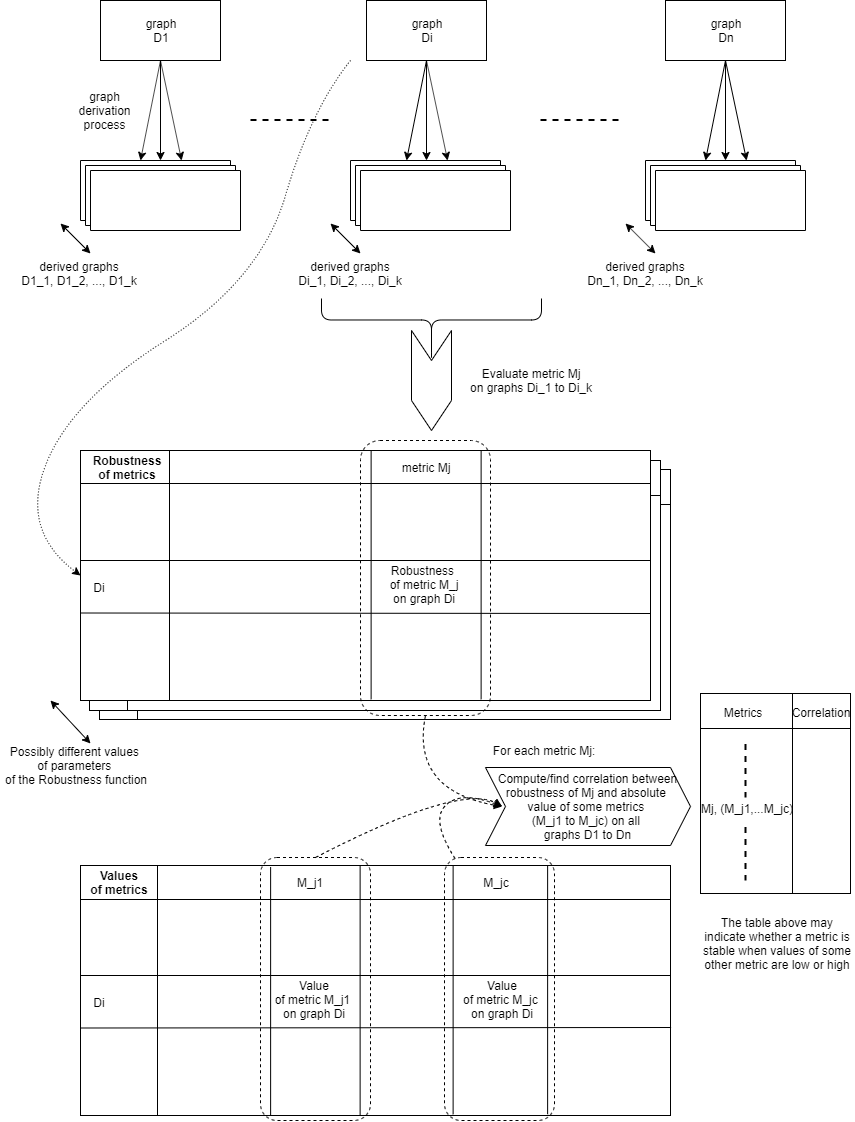
\includegraphics[width=16cm]{images/proposal_diagram1.png}
            \caption{An example of the evaluation process}
			\label{fig:example_eval}
            \end{figure}
	
	%I intend to use the programming language \textbf{Kotlin}, mainly for the following reasons. It is by nature similar to Java and can be used together with other Java code in a single project. Performance-wise, Kotlin is comparable to Java.
	%\begin{itemize}
	%    \item Concise, reducing the amount of boilerplate code
	%    \item Safe, preventing a significant number of errors
	%    \item IDE-friendly, allowing the IDE to help with software engineering
	%    \item Allows more functional constructs than Java
	%    \item Compiles to Java byte code and so preserves other important benefits of Java: Object-Oriented, platform-independent, extensible.
	%\end{itemize}
	
	\subsection*{Tasks}
	
	The following tasks need to be carried out to complete this project to the state described above.
	
	\begin{enumerate}
		
		\item Decide on the underlying graph framework, the programming language, tools and additional libraries to use for developing the software.
		
		\item Study graphs and their metrics to decide which metrics to carry out the described experiment on. This may depend on the complexity of the algorithm of the metric, usefulness of the metric in the graph research context, computing feasibility to evaluate the metric on large datasets and other factors.
		
		\item Study possible graph datasets and decide which graphs will be used in the experiment. Again this will take into account multiple factors such as availability of such datasets, commonness of the respective application area and others. This project intends to study robustness of graph metrics on graphs from different application areas.
		
		\item Devise a 'robustness' measure of a metric applied to a graph (possibly more measures for different aspects of robustness). This will likely be a function of a metric and an input graph, and will likely involve generating multiple graphs from the input graph that the robustness will be calculated for, for example by randomly deleting a small percentage of edges. For this, I will need to decide on what 'small perturbations' mean, which may as well be left as a parameter of the robustness measure.
		
		\item Build the platform to do the following:
		\begin{itemize}
		    \item Store, load and represent input graphs
		    \item Implement (or integrate existing) algorithms to compute graph metrics
		    \item Generate similar graphs, given an input graph, by making small changes or deletions
		    \item Implement the robustness function
		    \item Possibly, if suitable, produce visual results directly from the program
		\end{itemize}
		
		\item Execute the result, i.e. compute the robustness function value for chosen graph metrics and chosen input graphs, trying different values of parameters if appropriate.
		
		\item Evaluate the outcome and conclude the findings. Compare graph metrics in terms of their robustness based on the results of the experiment. Possibly compare the results of this experiment to the results of the paper by Bozhilova et al.
		
		\item Write up the dissertation.
		
	\end{enumerate}
	
	This project may additionally involve the use of secondary languages and platforms (such as Python, Jupyter notebook) for statistical analysis etc.

\section*{Success criteria}

	This project will be considered a success if I manage to complete the steps described above, primarily to execute the experiment and conclude any observations about graph metrics.
	
	\begin{enumerate}
	    \item Implement the experimental framework outlined above, using interesting datasets
	    \item Complete statistical analysis, as described in the~\nameref{subsec:evaluation} section
	    \item Deduce empirical observations about graph metrics
	\end{enumerate}
	
	The results of the experiment may also be compared to the results of the originating paper by Bozhilova, L. V., et al.

\section*{Possible extensions}

    The following ideas could be developed in case there is spare time during the implementation phase.
    
    \begin{enumerate}
        \item Wrap up and publish the project as an open-source library that can further be used by future projects.
        \item Develop a plugin to the Gephi graph visualisation software, to compute robustness of different metrics within the Gephi user interface.
        \item Produce a program, that will, given an input graph, be able to advise which metrics are more suited for describing such graph
    \end{enumerate}

\section*{Timetable}

	Planned starting date is 28 October 2019.
	
	\subsection*{Weeks 1 to 2}
	
		Research and read papers on similar topics. Read about graphs and network from relevant books.
		
		\textit{Milestone \textbf{8 November}: Fully understand the problem this project is solving and approaches possible.}
	
	\subsection*{Weeks 3 to 4}
	
	    Set up the working environment, decide on programming language and tools needed, repositories for code and dissertation, find and integrate relevant libraries, familiarise myself by creating toy programs on graphs.
	    
	    By taking various factors into account, decide on which metrics to analyse and which graph datasets to choose for the experiment. Use toy programs to estimate the complexity and feasibility of different algorithms on the datasets.
	    
	    \textit{Milestone \textbf{22 November}: Have a fully working setup of the programming environment with backup plans.}
		
	\subsection*{Weeks 5 to 6}
	
	    Devise the robustness measure(s) and mathematics behind the experiment. Write up the beginning of the dissertation.
	    
	    Beginning of the implementation: storing, loading and representing input graphs. Also, be able to generate pseudo-random graphs derived from an input graph.
	    
	    \textit{Milestone 6 December: Fully understand what robustness function the program will calculate and how.}
	
	\subsection*{Weeks 7 to 8}
	
	    Implement algorithms of the metrics to evaluate. Document the implementation.
	
		\textit{Milestone \textbf{20 December}: Working algorithm for each chosen metric}
		
    \subsection*{Weeks 9 to 10}
	
		Winter break, no work planned.
		
		%\textit{Milestone 3 January:}
	
	\subsection*{Weeks 11 to 12}
	
		Start implementation of the robustness measure(s).
		
		%\textit{Milestone \textbf{17 January}: }
		
	\subsection*{Weeks 13 to 14}
	
		Finish implementing the robustness measure(s) and a way to compare metrics. Write the Progress Report.
		
		\textit{Milestone \textbf{31 January}: Be able to calculate the robustness measure, for a given collection of similar graphs and a graph metric. Submit the Progress Report.}
	
	\subsection*{Weeks 15 to 16}
	
		Refine the robustness measure implementation. Integrate the individual parts of the implementation to create an executable program taking input parameters. If suitable, produce a statistical output from the program.
		
		\textit{Milestone \textbf{14 February}: Executable program}

	\subsection*{Weeks 17 to 18}
		
		Execute the evaluation (this may be very computationally expensive). Compare individual metrics and conclude results. Start writing the dissertation.
		
		\textit{Milestone \textbf{28 February}: Have some results of the evaluation}

	\subsection*{Weeks 19 to 20}
	
		Continue with carrying out the experiment. Over this period, focus mainly on writing the dissertation.
		
		%\textit{Milestone 13 March: Have some output}
	
	\subsection*{Weeks 21 to 22}
	
		Finish evaluation. Conclude experiment results. Continue writing the dissertation.
		
		\textit{Milestone \textbf{27 March}: Have the majority of the dissertation written up.}
	
	\subsection*{Weeks 23 to 24}
	
	    Ideally, work on extensions, or finish the implementation/evaluation if needed. Collect thorough feedback on the dissertation.
		
		\textit{Milestone \textbf{10 April}: Have a finished dissertation.}
	
	\subsection*{Weeks 25 to 26}
		
		The dissertation should be done by now. Polishing of the work if needed.
		
		%\textit{Milestone 24 April:}
		
	\subsection*{Weeks 27 to 28}
	
	    No work planned.
	    
	    \textit{Milestone \textbf{8 May}: Submit the dissertation}

\section*{Resource Declaration}\label{sec:resourcedeclaration}

    \subsection*{Personal resources}

    For the development and writing the dissertation, I will primarily use my personal laptop with an IDE such as IntelliJ IDEA. Source code and the written work will regularly be version-controlled in a git repository, backed up on GitHub and possibly other relevant online storage places. I accept full responsibility for this machine and the software and I have made contingency plans to protect myself against hardware and/or software failure, such as to fallback to using the MCS computers.

    \subsection*{Computing resources}

    This project requires the use of a high-performance computing resource, to run algorithms of evaluating metrics and their robustness on large (real-world or derived) graphs.
    
    Based on the paper by Bozhilova et al., calculating natural connectivity for a single node for a graph with ~7000 nodes takes ~88 seconds on a standard computer. Based on my toy example, calculating average betweenness centrality of ~2500 nodes takes ~8 minutes on my computer. Thus, assuming that computing a metric for an input graph of average size 5000 nodes takes ~1 hour, the pure computation time suggested by this Project Proposal would take the following time on a standard personal computer (approximated in the order of magnitude)
    \[(\sim 6\ \text{datasets}) \times (\sim 6\ \text{metrics}) \times (\sim 50\ \text{derived graphs}) \times (\sim 1\ \text{hour}) \approx 75\ \text{days}\]
    
    The following resource has been granted permission for and will be used to parallelise the process and thus significantly speed up the computation time:
    
    \begin{adjustwidth}{1cm}{}
    	Resource: a computing facility (such as one of the servers \textit{yellow, nile,} or \textit{rio})\\
    	Institution: Systems Research Group (\url{https://www.cl.cam.ac.uk/research/srg/})\\
    	Sponsor: Dr Andrew Moore (\url{andrew.moore@cl.cam.ac.uk})
    	
    	This requires setting up a Computer Laborarory account.
	\end{adjustwidth}
    
    An alternative to this is Amazon Web Services or Google Cloud with free credits for students.
    
    \subsection*{Datasets}
    
    Graph datasets are available and will be obtained from either of the following sources (or others):
    
    \begin{itemize}
        \item Stanford Large Network Dataset Collection: \url{https://snap.stanford.edu/data/}
        \item STRING Database: \url{https://string-db.org/}
    \end{itemize}

\end{document}
